\chapter{轮式机器人决策系统}\label{introduction}
\section{问题定义}
本文研究的轮式机器人决策问题是以ICRA DJI 机甲大师人工智能挑战赛(ICRA DJI RoboMaster AI Challenge)为基础的。该问题的定义为:在给定的室内有边界的场地内,由敌我双方各使用两台搭载有传感器与弹丸发射机构的轮式机器人在场地内进行对战。挑战赛比赛场地,是一个长为8 米、宽为5米的长方形区域,主要包含启动区、补给区、防御加成区、障碍块区和保护围挡区,如图\ref{field}所示。

\begin{figure}[htb]
  \centering
  % Requires \usepackage{graphicx}
  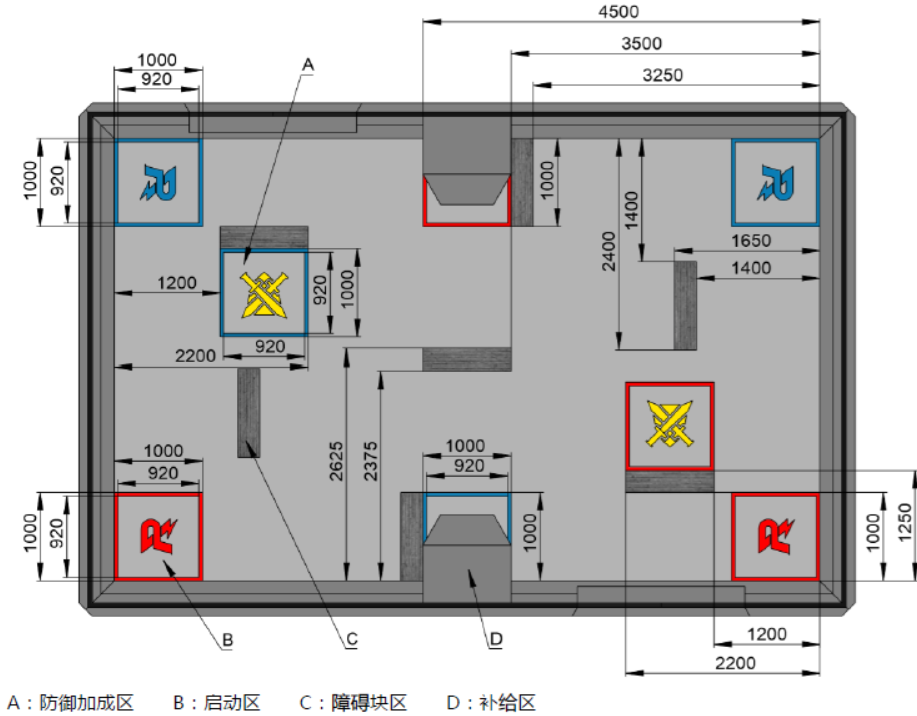
\includegraphics[width=\textwidth]{figures/field.png}
  \caption{挑战赛场地}\label{field}
\end{figure}

\begin{figure}[htb]
  \centering
  % Requires \usepackage{graphicx}
  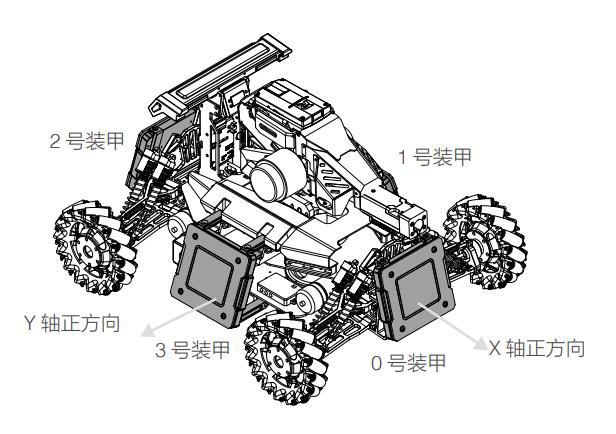
\includegraphics[width=\textwidth]{figures/robot.png}
  \caption{轮式机器人与装甲模块}\label{robot}
\end{figure}


敌我双方一到两台轮式机器人分别从各自图\ref{field}的B启动区启动,在挑战赛场地内进行全自主的对抗。在挑战赛场地内,设置诸多不可移动的灰色障碍物如图\ref{field}的C障碍块区所示。同时设置了A防御加成区,轮式机器人在这一区域中停留超过5s后即可获得伤害减半的buff持续时间30s。在D补给区己方轮式机器人可以获得弹药补给。

轮式机器人可以搭载激光雷达、摄像头、UWB、超声波等多种传感器。轮式机器人四周各装有装甲模块。装甲模块装有红蓝两种色彩的LED用以区别敌我,同时装有压力传感器以检测车身是否被击中,并计算剩余血量。装甲模块如图\ref{robot}所示。

\section{决策系统架构}
\subsection{架构概述}\label{system}
在应用与实践中,我们总结形成一套基于ROS的轮式机器人的控制软件系统。该架构包括该架构包括驱动模组、感知模组、规划模组、控制模组和决策模组。

驱动模组通过选取适合的驱动软件包调用摄像头、雷达、声呐、UWB等传感器数据以获取轮式机器人实时环境信息;通过解析步兵战车通信协议,构造串口驱动类,实现对轮式机器人的控制。感知模组通过雷达、声呐、UWB等传感器信息实现地图构建、实时定位;通过轻量级深度神经网络:SSD-MoblieNets达到了在Jetson TX2开发组件上的实时目标定位与追踪。规划模组主要通过优化Navigation功能包,实现了轻量级的路径规划器,使轮式机器人在有限的计算资源下,完成了全自主巡航功能。控制模组使用了离散式增量PID控制,其结合经典控制理论与SIMULINK仿真技术,实现了对目标物的低超调高速自动追踪。

\subsection{模组通信}
我们使用ROS的Publish/Subscribe机制实现各个模组之间的通信。各个模组的数据流如图\ref{dataflow}所示。各个ROS消息结点的消息传递关系如图\ref{topic}所示。

驱动模组负责将轮式机器人状态、比赛进度、电机里程计数据、摄像头图像、激光雷达云点阵、UWB定位等数据推送给感知模组。感知模组使用目标检测、物体识别与实时定位算法,确定当前己方轮式机器人与敌方轮式机器人在场地中的位置等状态信息。决策系统根据状态信息,将决策己方轮式机器人做出的反应动作,即目标位置与姿态,并将其推送给规划模组以经行路径规划。规划模组根据目标位置与姿态使用导航算法得出底盘与云台运动的速度等数据。这些数据由控制模组处理后,通过驱动模组中的串口驱动发送给下位机执行。

\begin{figure}[htb]
  \centering
  % Requires \usepackage{graphicx}
  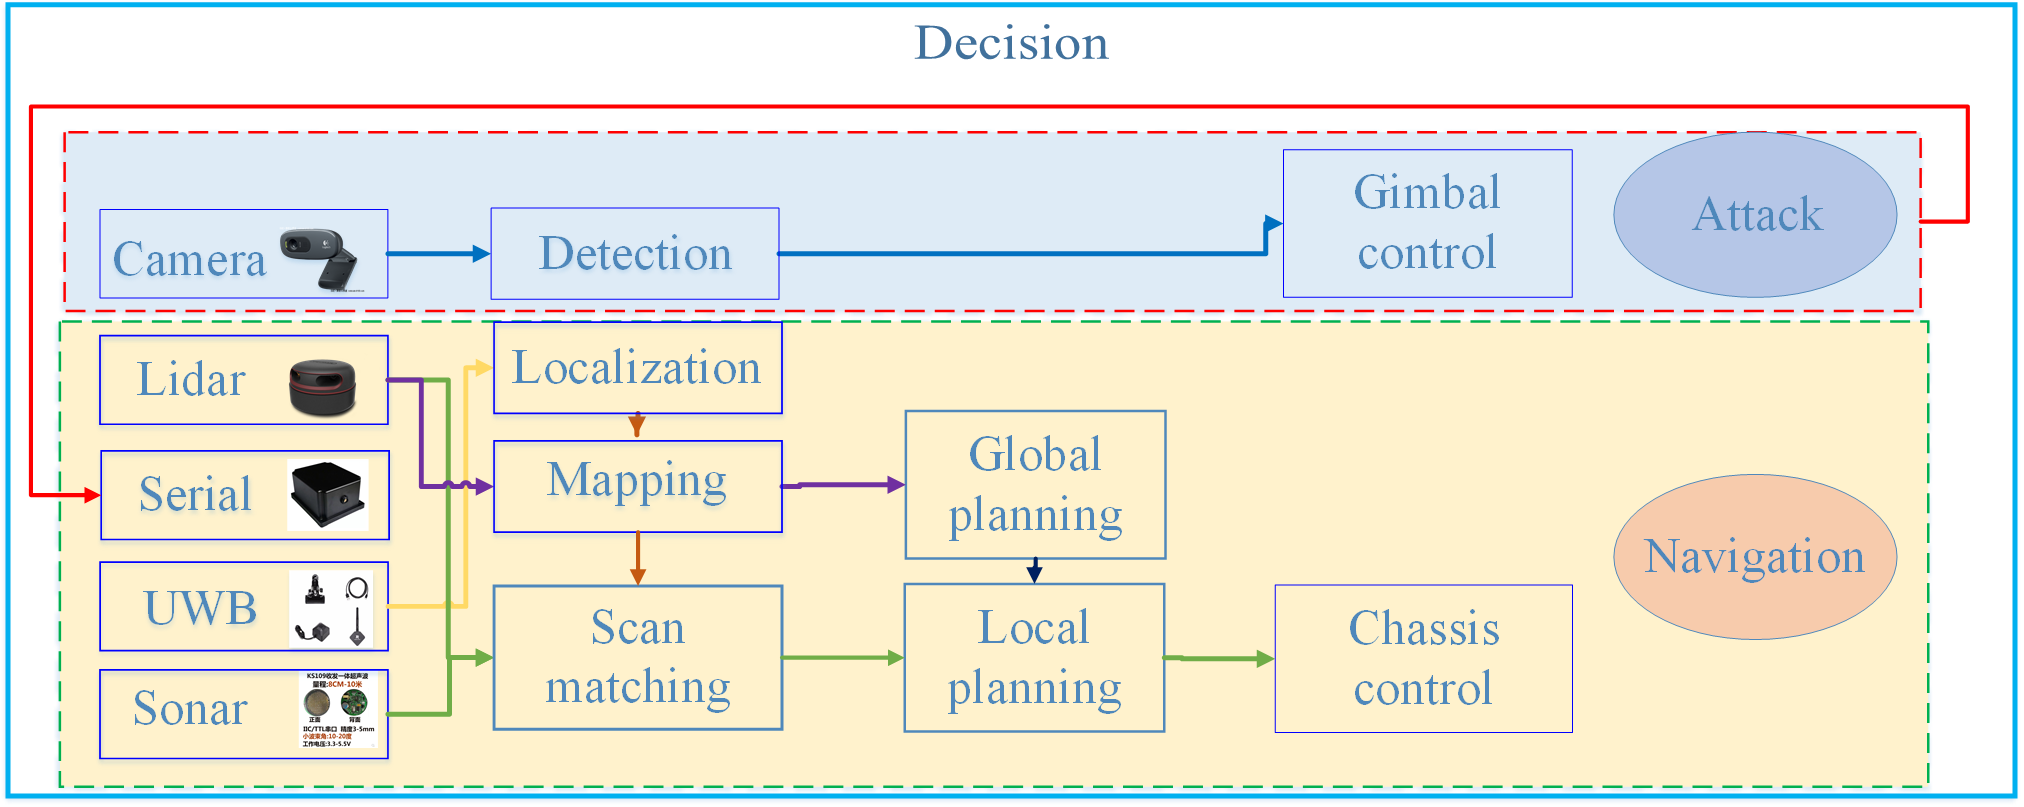
\includegraphics[width=\textwidth]{figures/dataflow.png}
  \caption{模组通信数据流}\label{dataflow}
\end{figure}

\begin{figure}[htb]
  \centering
  % Requires \usepackage{graphicx}
  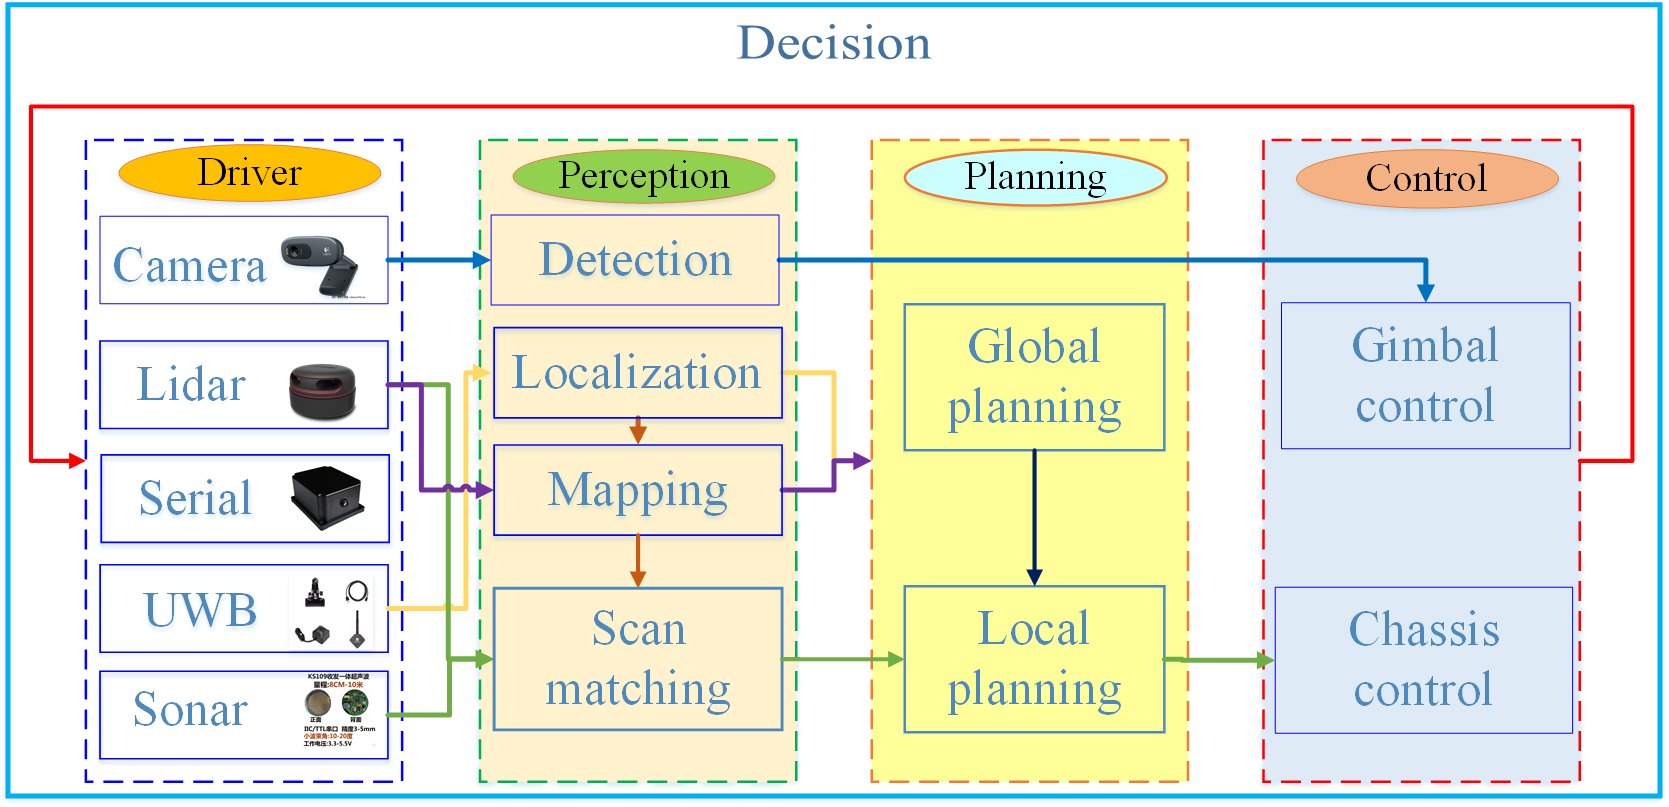
\includegraphics[width=\textwidth]{figures/function.png}
  \caption{模组功能}\label{function}
\end{figure}

\begin{figure}[htb]
  \centering
  % Requires \usepackage{graphicx}
  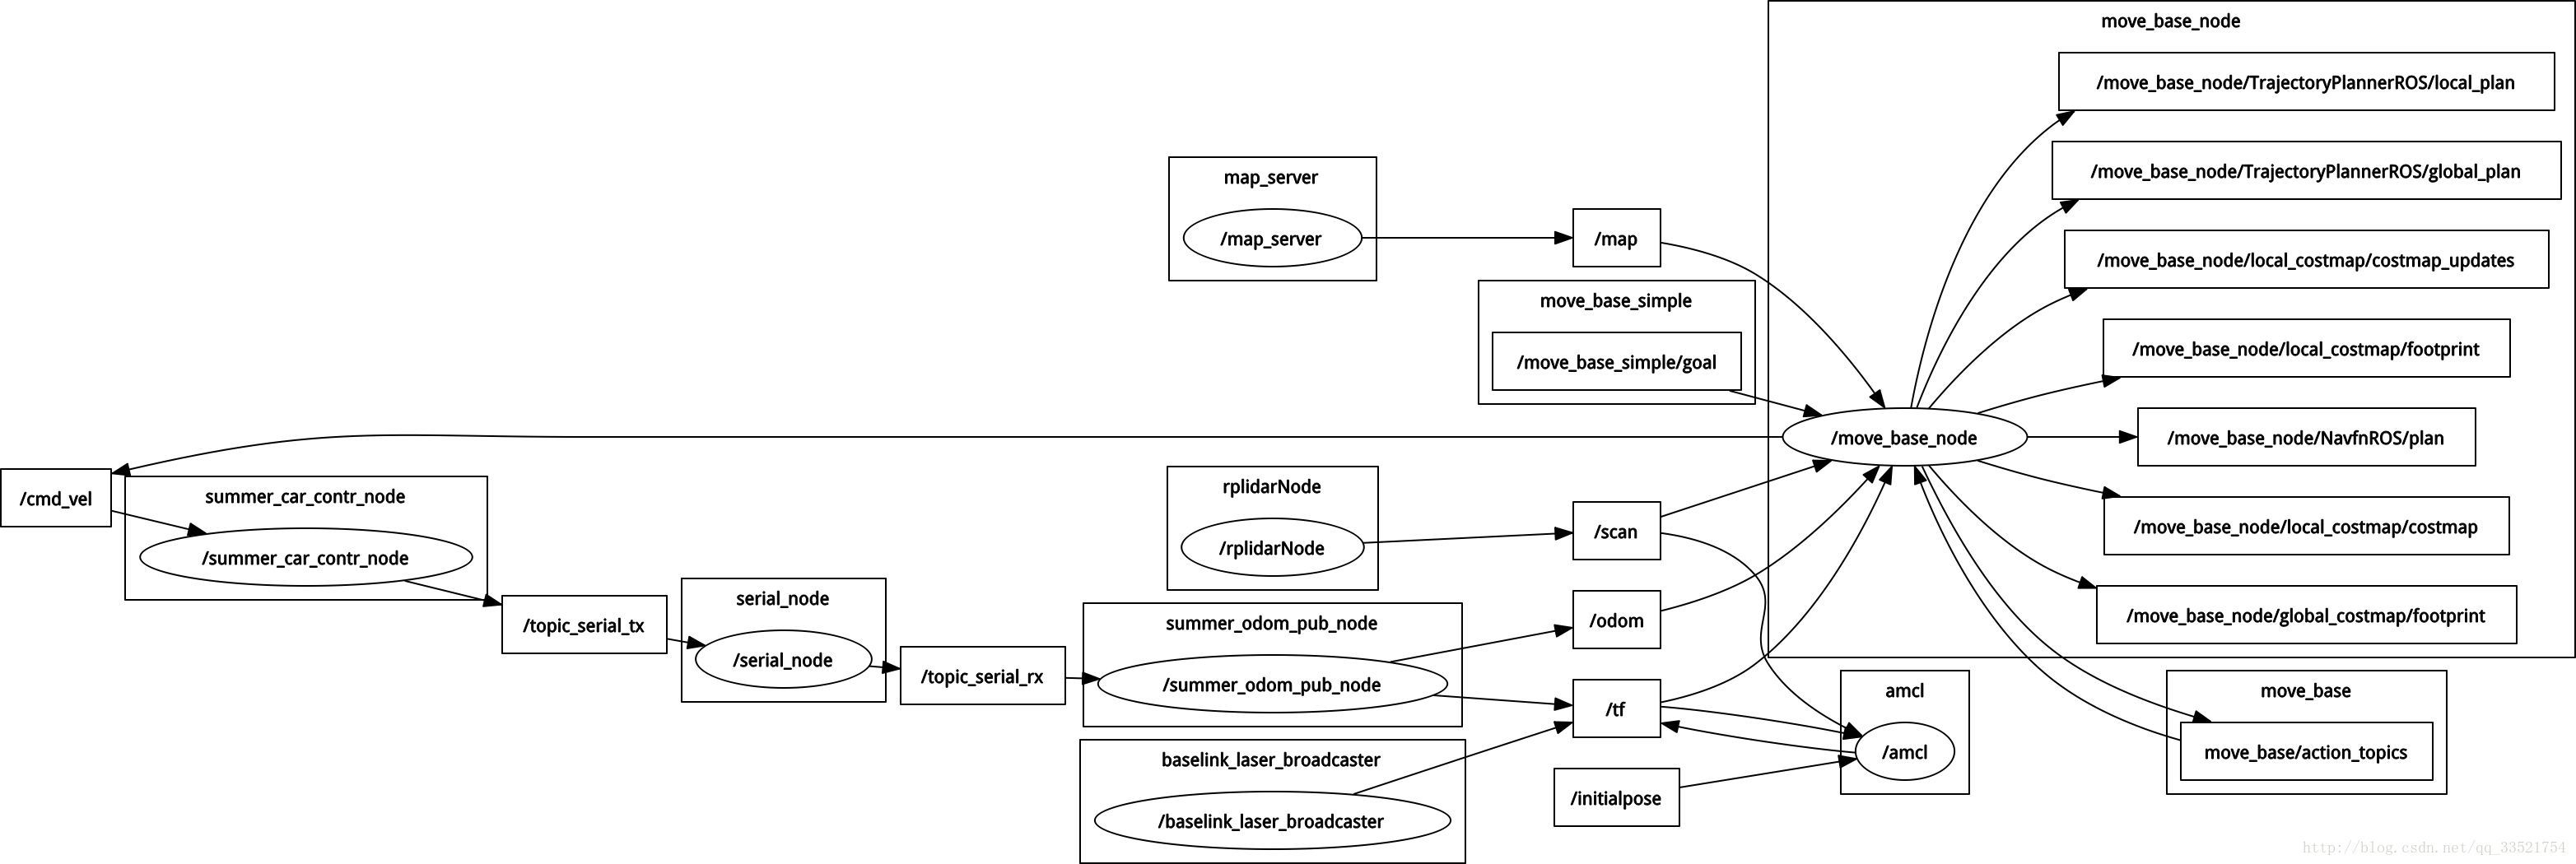
\includegraphics[width=\textwidth]{figures/topic.png}
  \caption{ROS消息结点关系}\label{topic}
\end{figure}

\subsection{模组功能}
总体而言,决策系统主要依赖改软件系统的两大功能:导航和攻击,如图\ref{function}所示。导航功能主要负责在挑战赛环境下自主避障、路径规划。攻击功能主要负责实时检测、追踪和打击敌方目标。决策系统建立在在可靠的导航与攻击功能上,实际上负责协调导航与攻击功能模块的交互。决策系统可以视为模组功能沟通与协调的结点,通过接收感知信息以合理地调用各个模组功能。

\section{决策系统设计}
在ROS平台上,决策系统实际上是一个消息处理结点,它通过处理轮式机器人的感知信息,向轮式机器人发布控制命令,已协调调用各个模组的功能,从而能够实现轮式机器人全自主的巡航、索敌、追踪与打击,如图\ref{decision} 所示。
\begin{figure}[htb]
  \centering
  % Requires \usepackage{graphicx}
  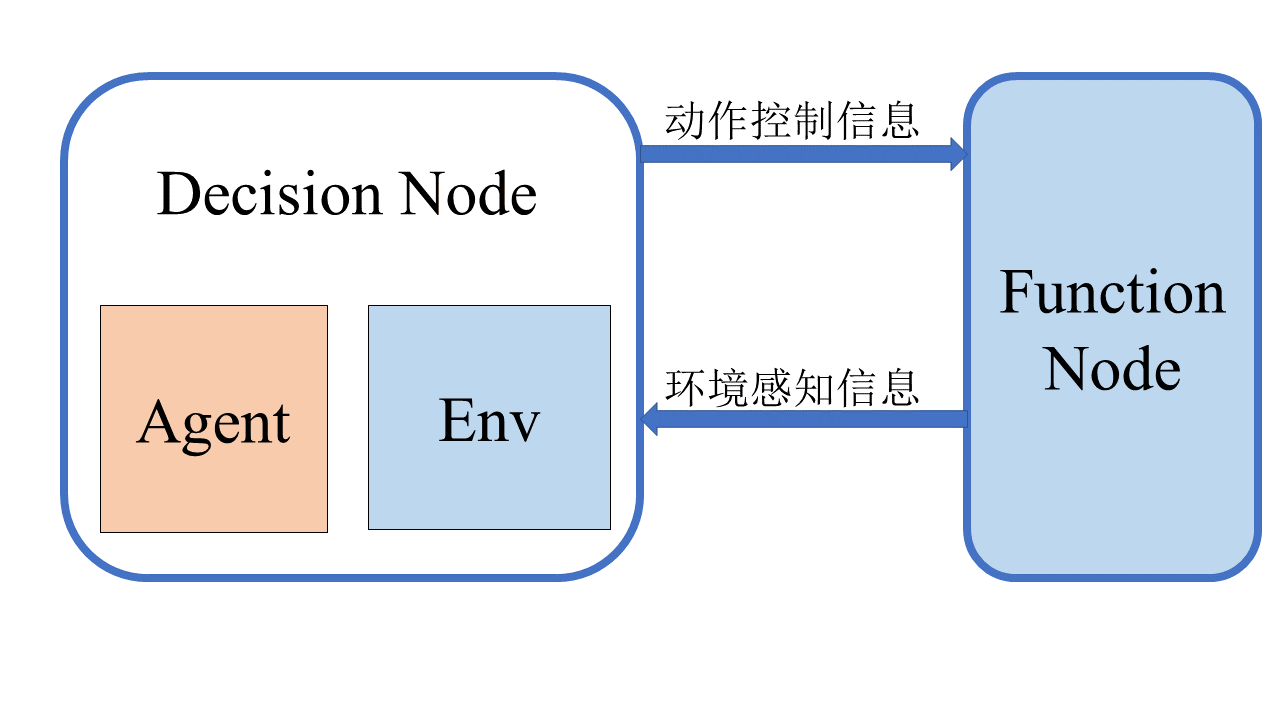
\includegraphics[width=\textwidth]{figures/decision.png}
  \caption{决策结点消息交互接口}\label{decision}
\end{figure}

在决策系统设计时,考虑到可扩展性、在虚拟环境与真实环境下的适应性、与深度强化学习算法的兼容性,我们使用OpenAI gym标准接口封装了轮式机器人感知、通信与控制功能,构建一个环境适配器类env,从而实现了智能体agent与环境env的交互。智能体agent通过状态state、动作action和奖励reward与环境env进行交互,从而进行训练,如图\ref{agentenv} 所示。
\begin{figure}[htb]
  \centering
  % Requires \usepackage{graphicx}
  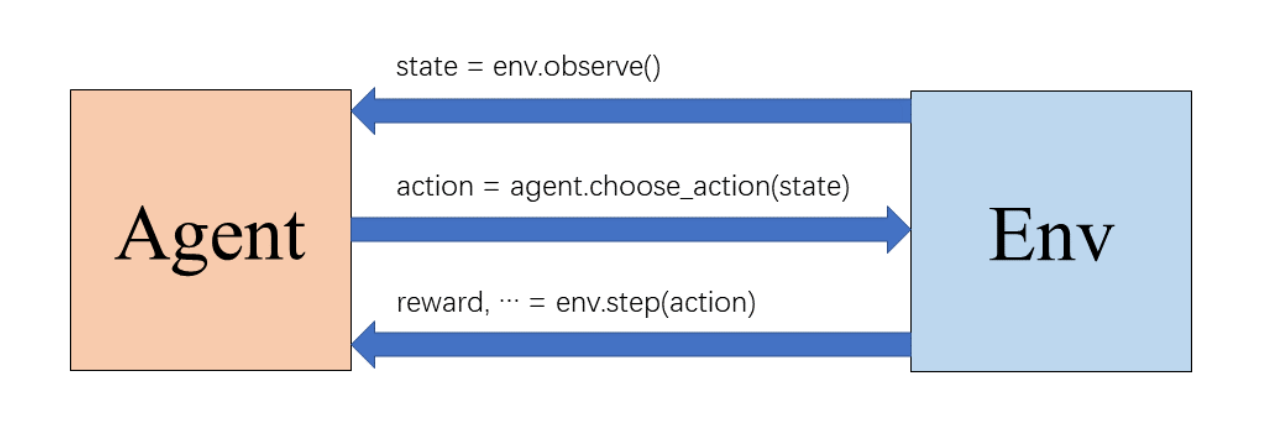
\includegraphics[width=\textwidth]{figures/agentenv.png}
  \caption{轮式机器人智能体与环境交互接口}\label{agentenv}
\end{figure}

按照OpenAI gym标准,我们将复杂的轮式机器人感知与控制抽象为智能体agent和环境env之间交互的三个函数:
\vspace{-10pt}
\begin{enumerate}
	\item 感知环境,$\text {env.observe}$。同步消息机制。输入为空,输出为轮式机器人智能体当前在环境中感知的状态。
	\item 动作决策,$\text {agent.choose action}$。同步消息机制。输入为轮式机器人智能体当前状态,输出为轮式机器人智能体自主做出的动作响应决策。
	\item 执行动作,$\text {env.step}$。同步消息机制。输入为轮式机器人智能体做出的动作响应,输出为环境反馈给轮式机器人智能体的奖励或惩罚和下一步。
\end{enumerate}

应用适配器模式的思想,将智能体agent做出动作决策与环境env交互解耦。环境env隐藏了决策系统结点与ROS目标识别、定位、移动控制等其他消息结点的交互细节,使智能体agent 只关心与环境env的交互。

环境env无需关心智能体agent的实现细节,通过继承env,可以是智能体在仿真轮式机器人环境与真是轮式机器人环境之间切换,从而提高了工作效率,减少了实验好耗时。

同样的,智能体agent无需关心环境env与轮式机器人的交互细节,通常来说,智能体agent只需要实现输入一个状态向量或矩阵$s$ 时,输出一个动作响应向量或矩阵$a$,就能够与环境env进行交互。因此,智能体agent可以在不同的强化学习算法、不同的神经网络模型之间灵活切换,甚至可以替换为非强化学习模型,如确定性有限状态机和行为树。

\subsection{确定性有限状态机}\label{dfa}
决策系统上我们使用人工设计的确定性有限状态机作为本文实验的基线,通过对所有可能出现的情况与相对应的行为来构建有限状态机,其中状态图如图\ref{state}所示,活动图如图\ref{activity} 所示,我们成功地对轮式机器人的行为策略进行规划,并在实际实践中取得良好的效果。

\begin{figure}[h]
  \centering
  % Requires \usepackage{graphicx}
  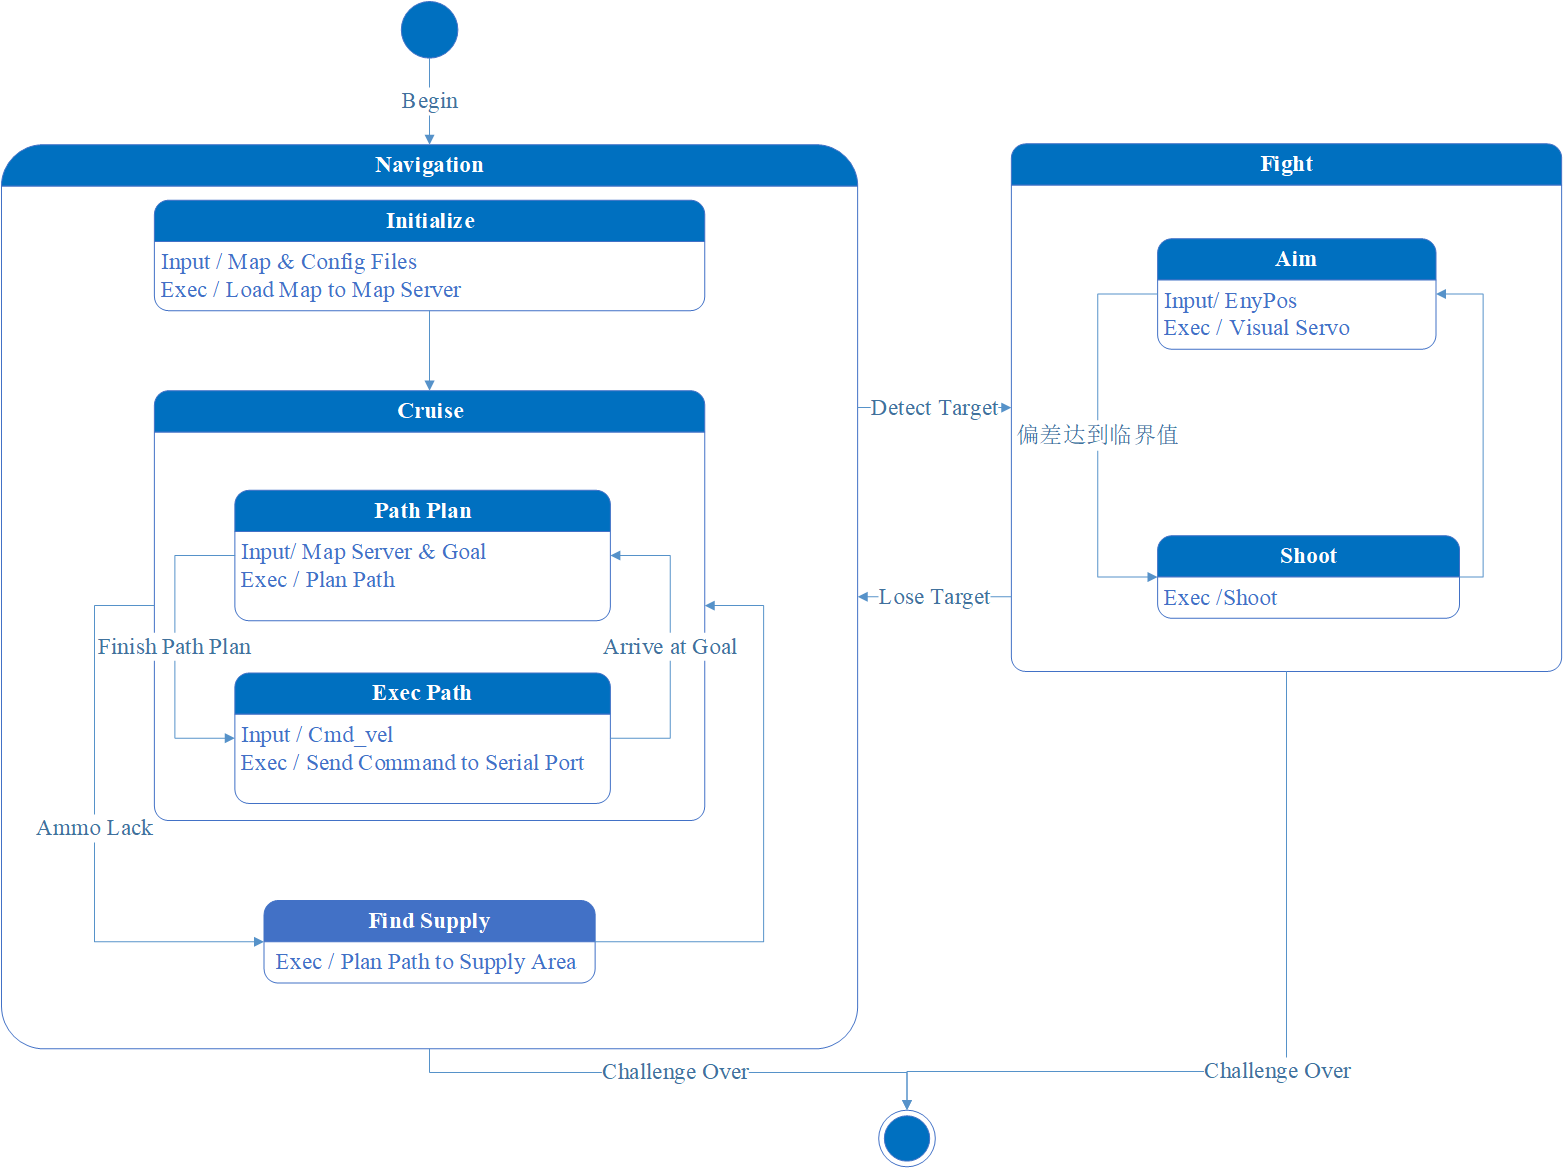
\includegraphics[width=\textwidth]{figures/state.png}
  \caption{轮式机器人确定性有限状态机}\label{state}
\end{figure}

\begin{figure}[h]
  \centering
  % Requires \usepackage{graphicx}
  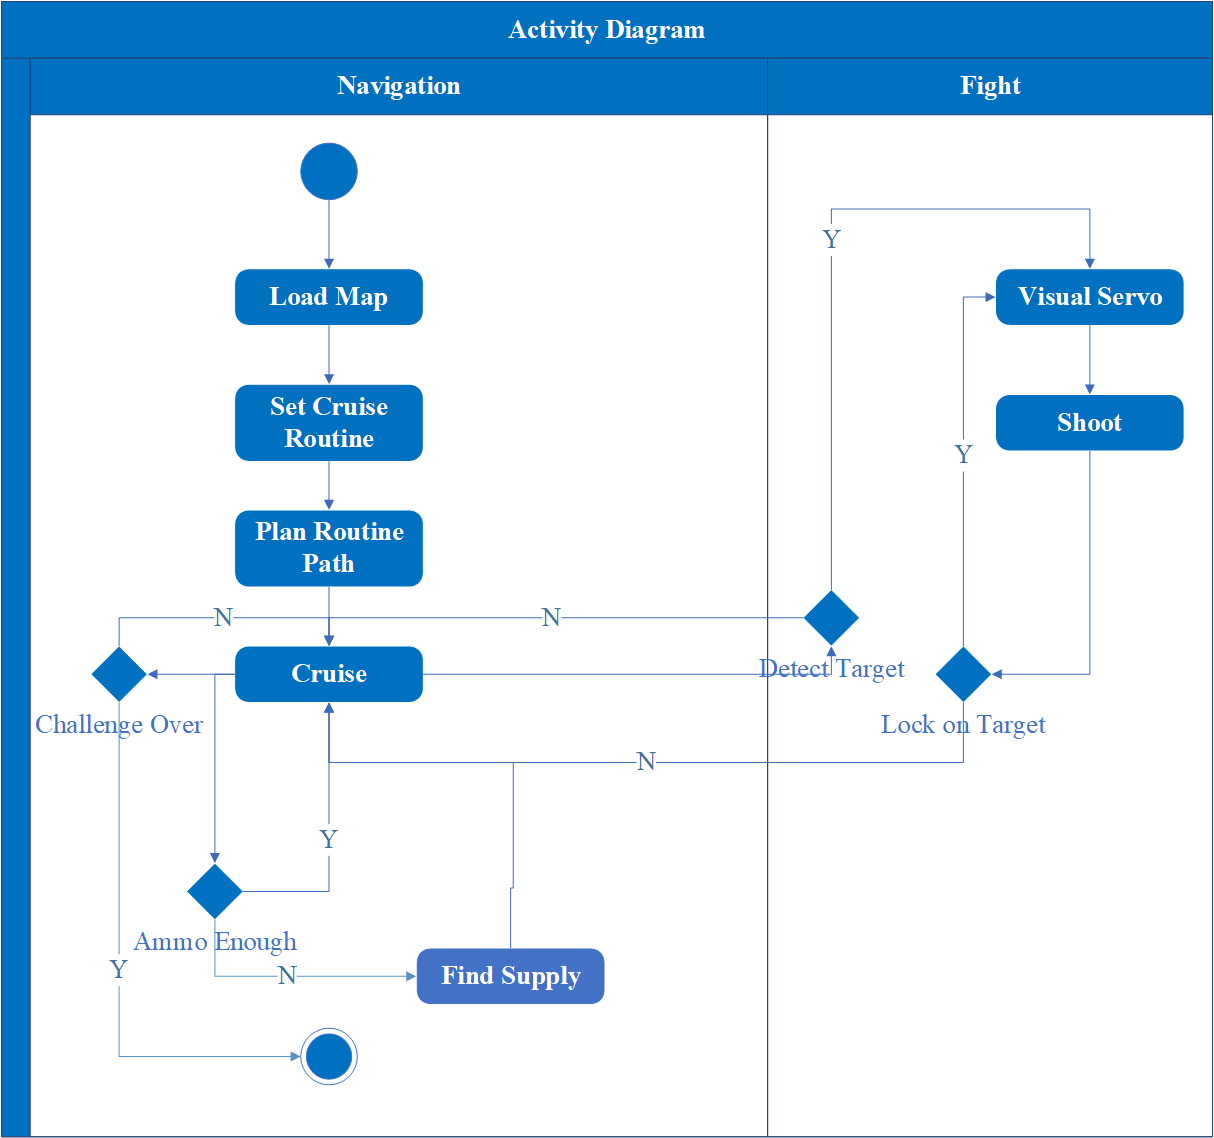
\includegraphics[width=\textwidth]{figures/activity.png}
  \caption{轮式机器人活动图}\label{activity}
\end{figure}
